\paragraph{Pure MC Systematics \\}

Deriving uncertainties is challenging for q/g tagger that based on the track multiplicity, especially in the higher \pt\ regime partly due to a lack of statistics beyond 1 TeV, where less gluon jets as they are usually produced at lower masses than quark jets.  This leads to an issue of the equations that require an average number of tracks in quark or gluon jets to do the calculations.

The fraction of jets labeled as quark/gluon initiated jets is defined as $f^f_q$/$f^c_g$ where the superscript $f$($c$) denotes the jet with higher (lower) $\eta$ compared to each other in simulated dijet events. The fractions are extracted from parton distribution functions convoluted with matrix element calculations. The number of events of charged tracks in higher $\eta$ jet can be described by the following system of equation:

% \cite{ATL-PHYS-PUB-2017-009}:

\begin{eqnarray}
\langle n^f_{\mathrm{charged}} \rangle = f^f_q \langle n^q_{\mathrm{charged}}\rangle + f^f_g\langle n^g_{\mathrm{charged}}\rangle\, 
\langle n^c_{\mathrm{charged}} \rangle = f^c_q \langle n^q_{\mathrm{charged}}\rangle + f^c_g\langle n^g_{\mathrm{charged}}\rangle\, .
\end{eqnarray}

These equations require two samples with different fractions of quark and gluon jets, it is valid theoretically even at high \pt. However, due to the fact that the fractions of gluon jets become so small at high \pt~, the equations are less useful at high \pt regime. The main uncertainties are from MC mismodelling and reconstruction of charged 
tracks inside jets, as the the separation between tracks are almost of the same order as the detector resolution. Thus the tagger efficiency depends on the good track resolution for an accurate value of $n_\mathrm{track}$, and limited by the statistics obtained.

They systematic uncertainty can be estimated by using pure MC and is supposed to be large but smaller than from the data at the edges of the mass range. Where there is no statistics limited, such as the centre of the \pt\ distribution, such technique is proved to be the best choice. To extend the uncertainties to higher \pt~regime,  particle level effects and MC reconstruction effects are taken into account as these uncertainties are to $in-situ$ ones thus is reasonable to move away when doing an extrapolation procedure.

The procedure is performed at constant \pt\ ranges, as $n_\mathrm{track}$ depends only on \pt\ and the parton type that initiating jets, uncertainties can be computed by comparing the distribution of $n_\mathrm{track}$ in bins of jet \pt~, which generated from different simulation models. Thus different type of MC generators could introduce underlying uncertainties to the results. Details on different types of uncertainties and the samples used to estimate them are described in Section.~\ref{sec:QG-syst}. Six working points (10\%, 25\%, 40\%, 50\%, 60\% and 75\%) are provided for fixed efficiency curves.


%\paragraph{Track Systematics\\}
%
%Nominal \pythia~samples are used for estimating track systematics, four track systematics are considered, labeled as: 1.track reconstruction efficiency. 2.uncertainty on the rate of reconstructing fake tracks passing the Loose track selection. 3.uncertainty for weak modes in the detector alignment. 4.TIDE efficiency. As shown in Figure~\ref{fig: ratioplots}, no variation for weak modes in detector alignment, and the remaining uncertainties are small.
%
%
% \begin{figure}[!htb]
%   \centering
%    \subfloat[]{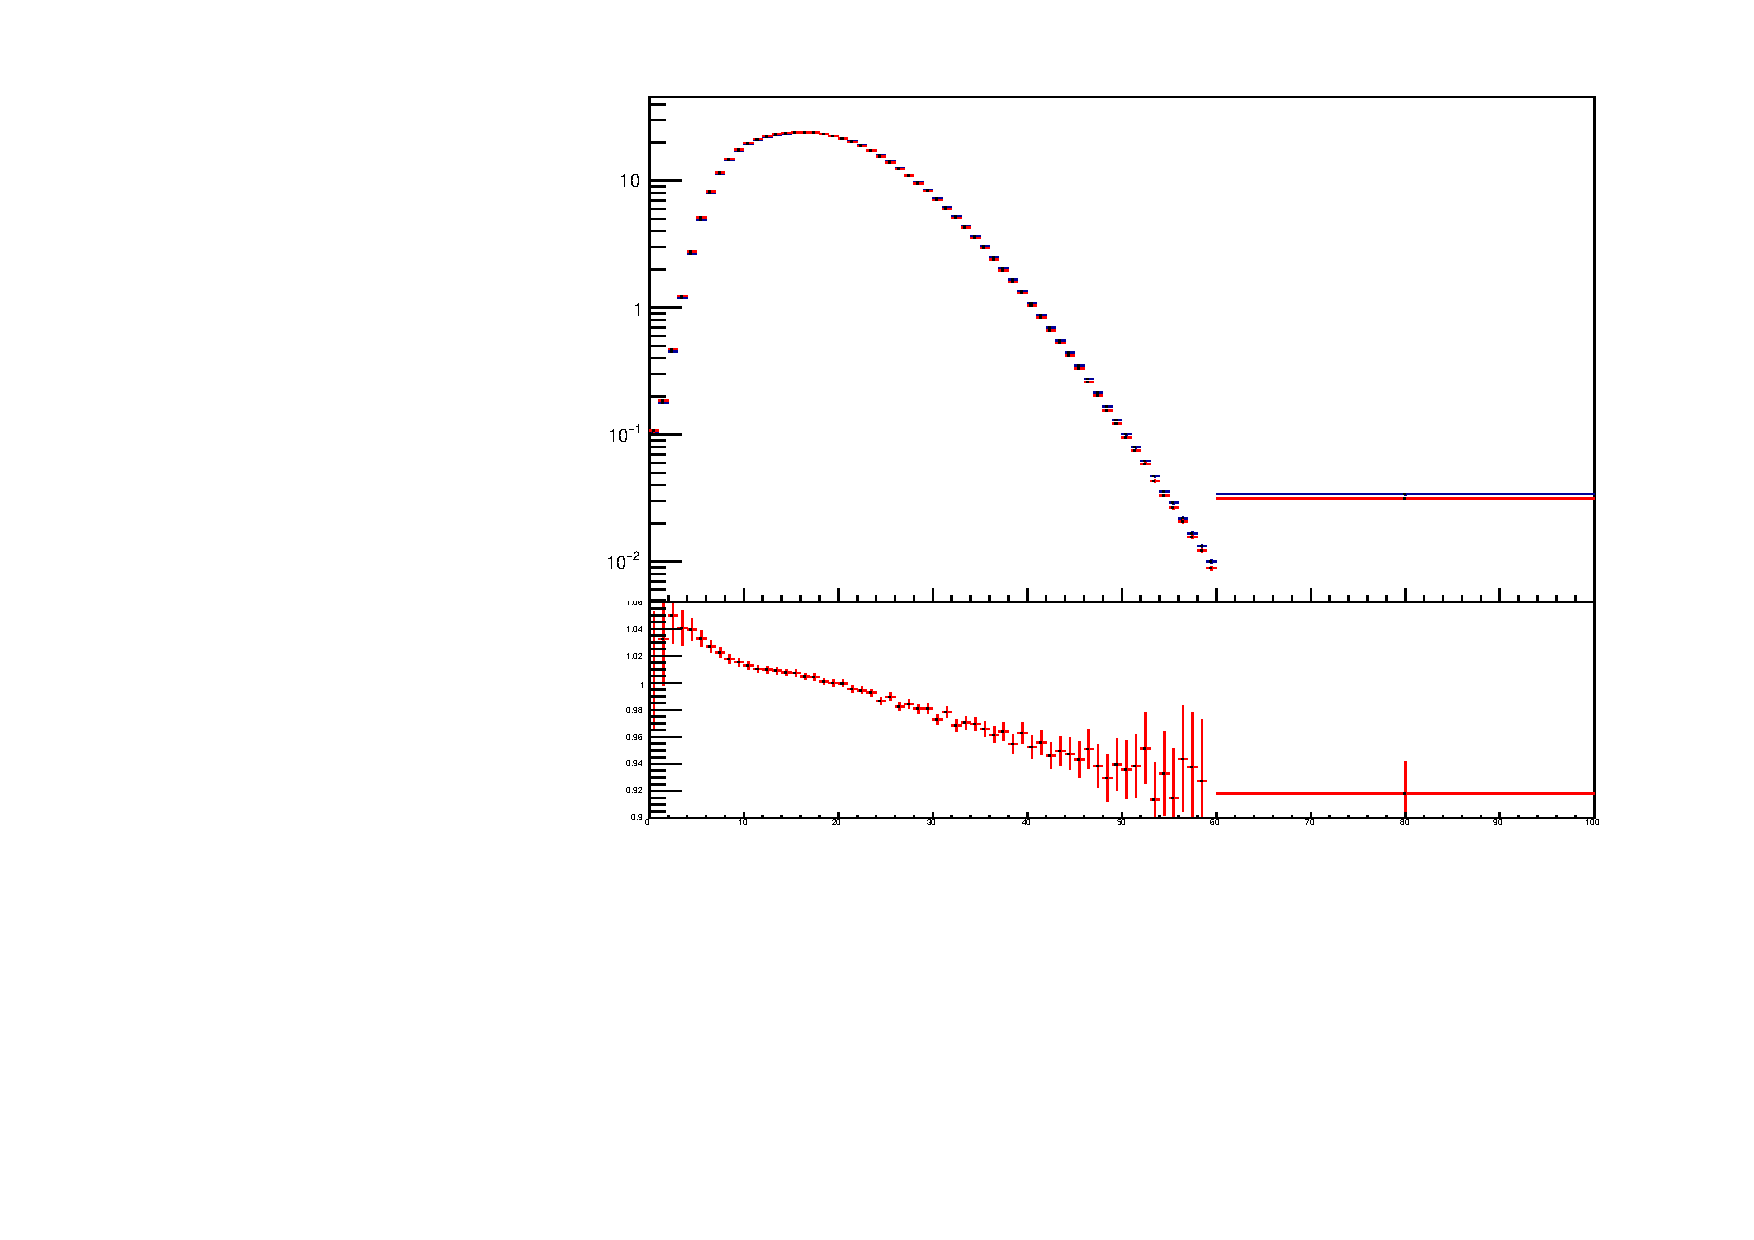
\includegraphics[width=0.48\columnwidth]{fig/Systematics/Tracking1.pdf}} 
%    \subfloat[]{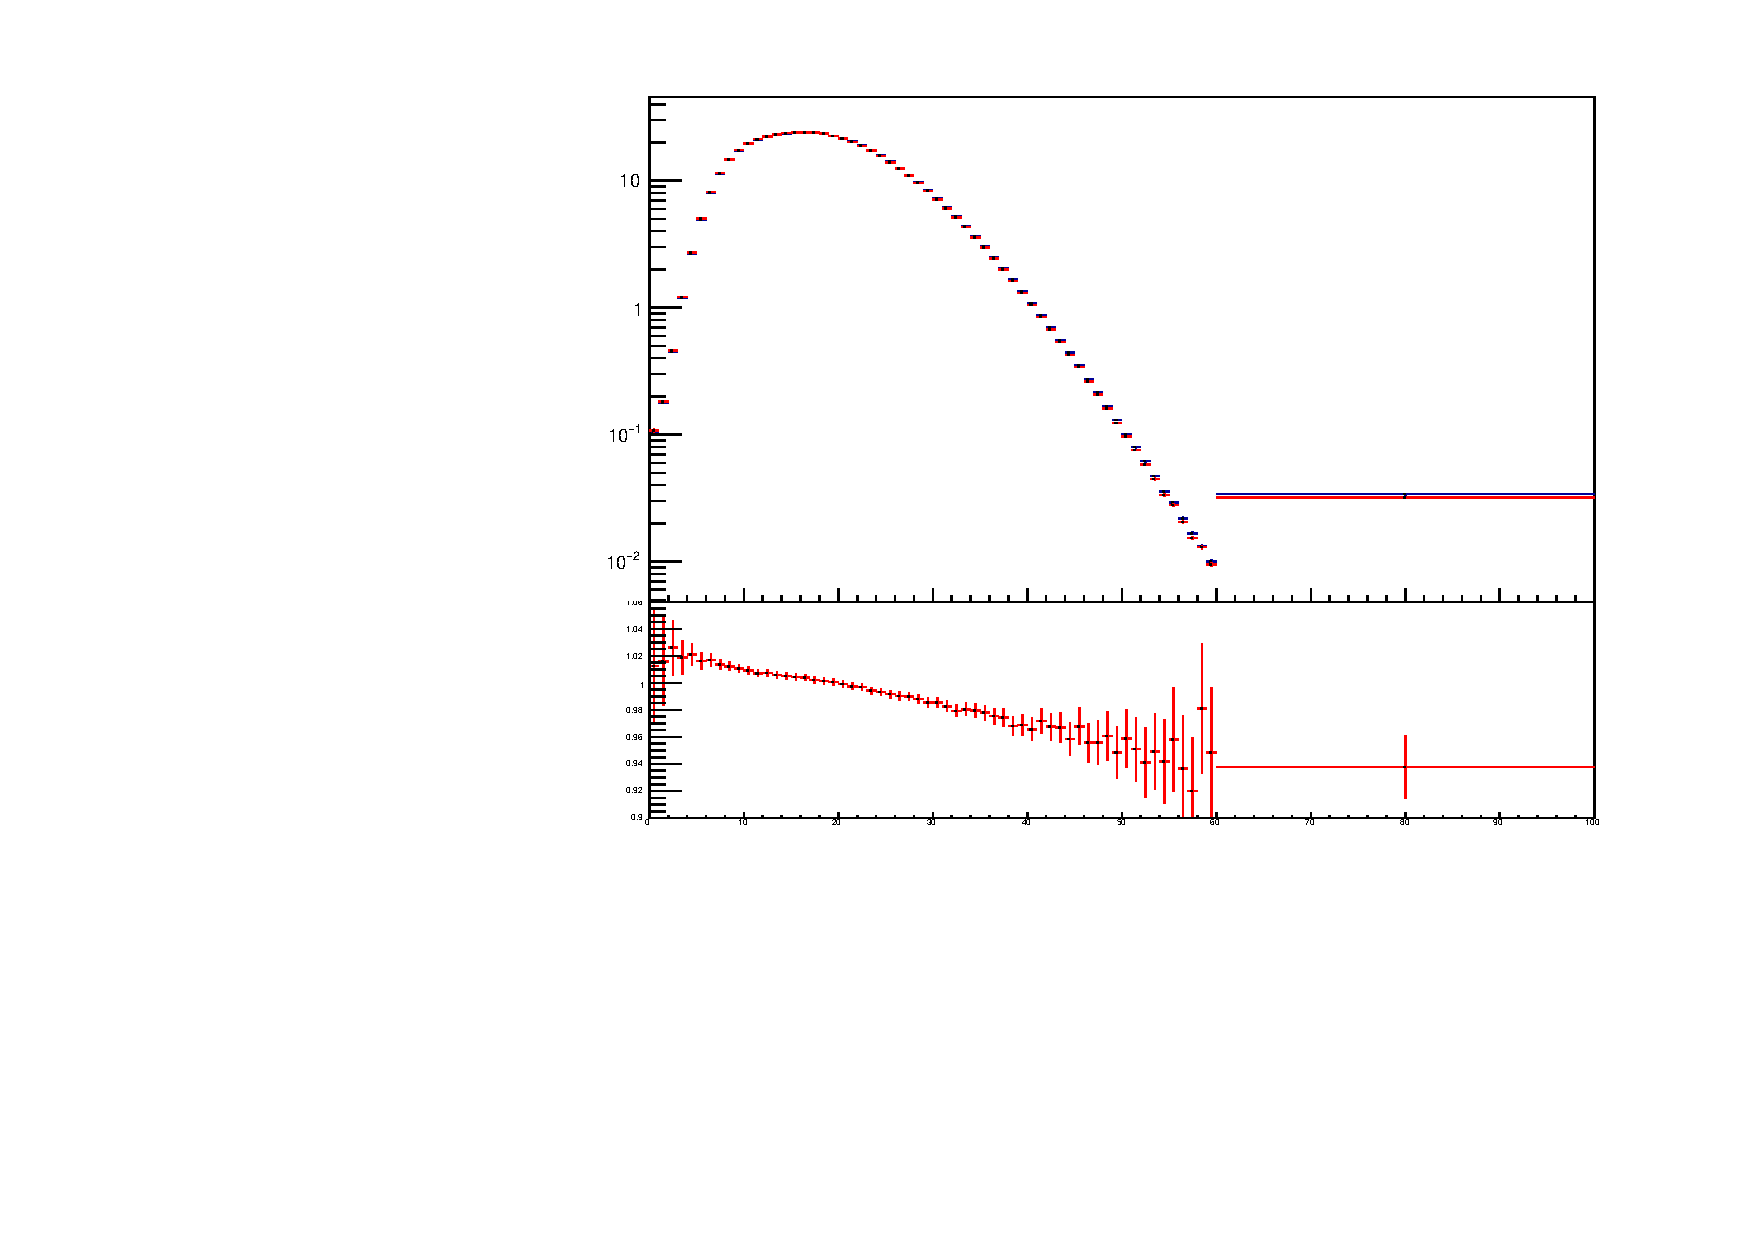
\includegraphics[width=0.48\columnwidth]{fig/Systematics/Tracking2.pdf}}   
%   \\
%    \subfloat[]{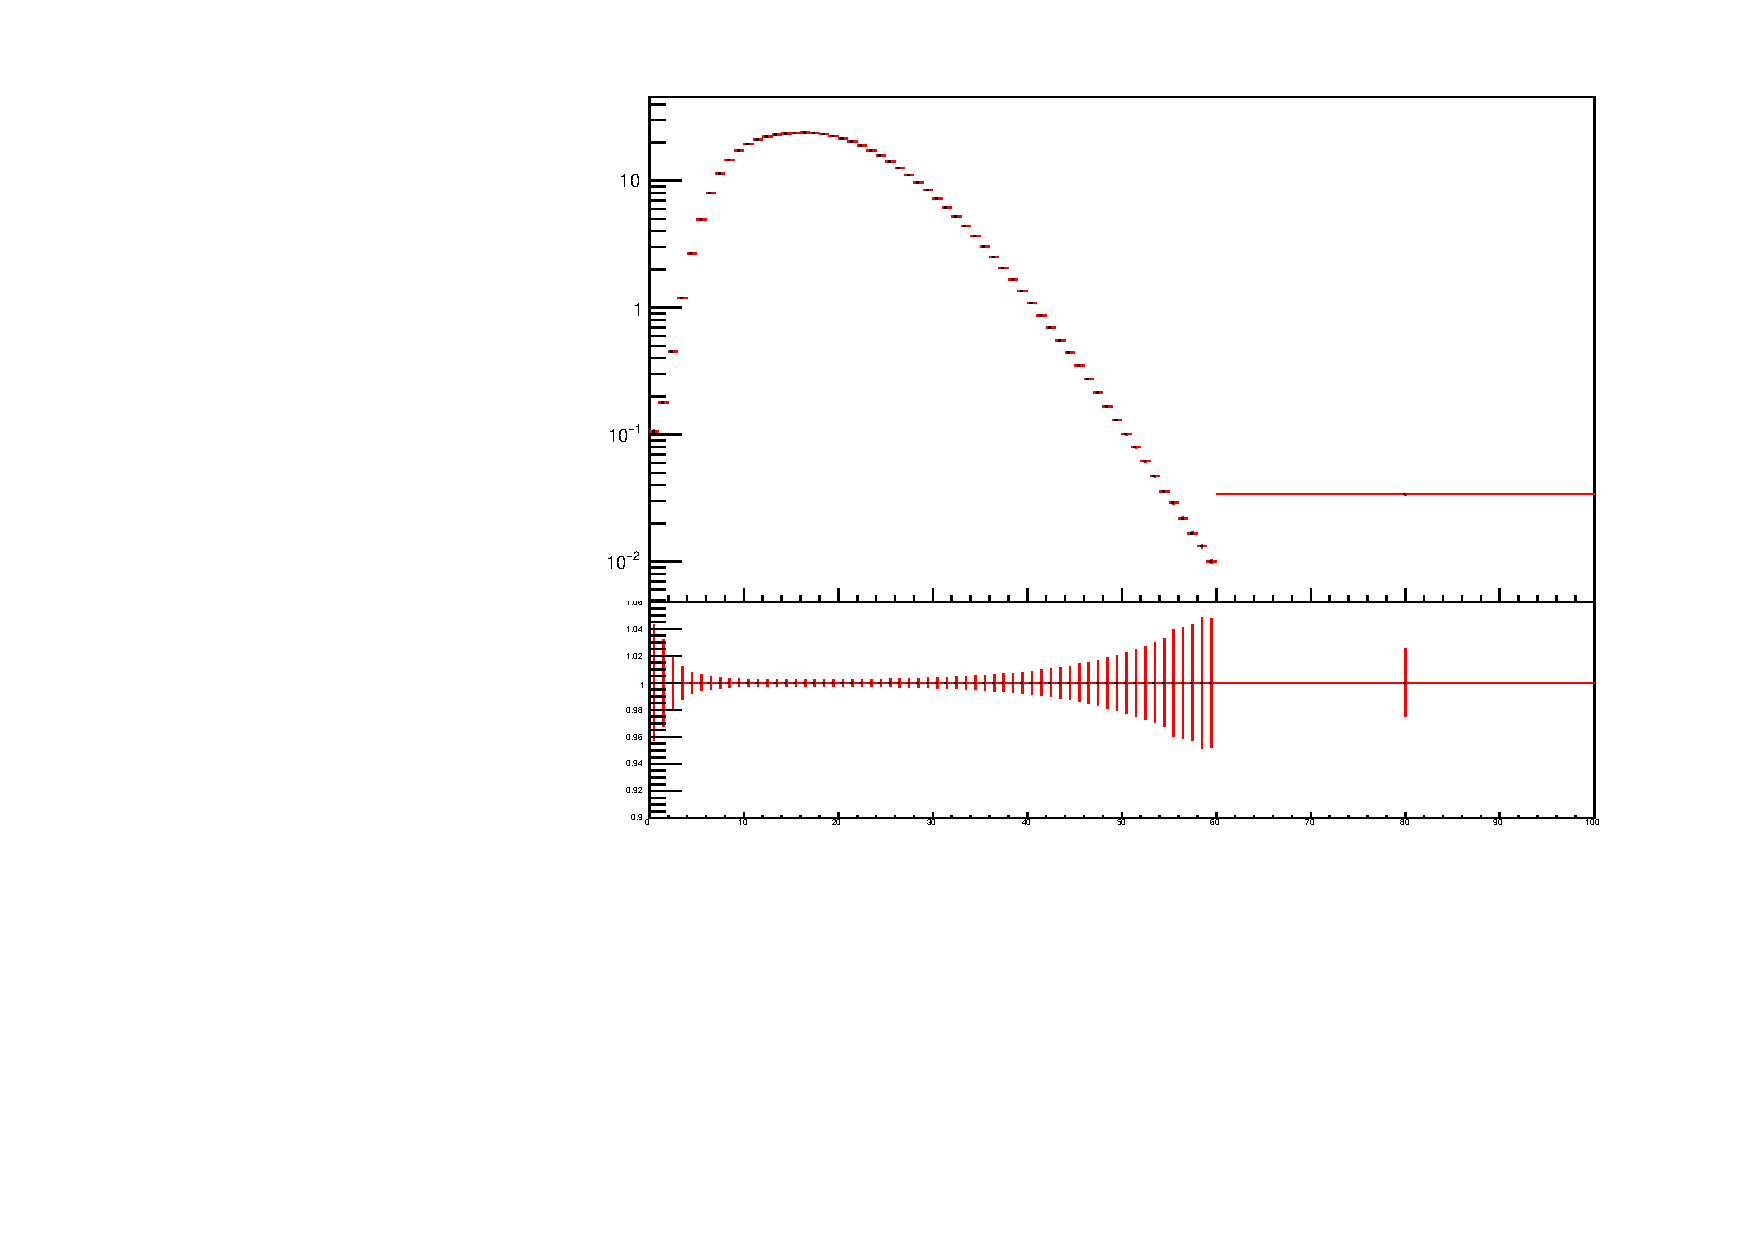
\includegraphics[width=0.48\columnwidth]{fig/Systematics/Tracking3.pdf}}
%    \subfloat[]{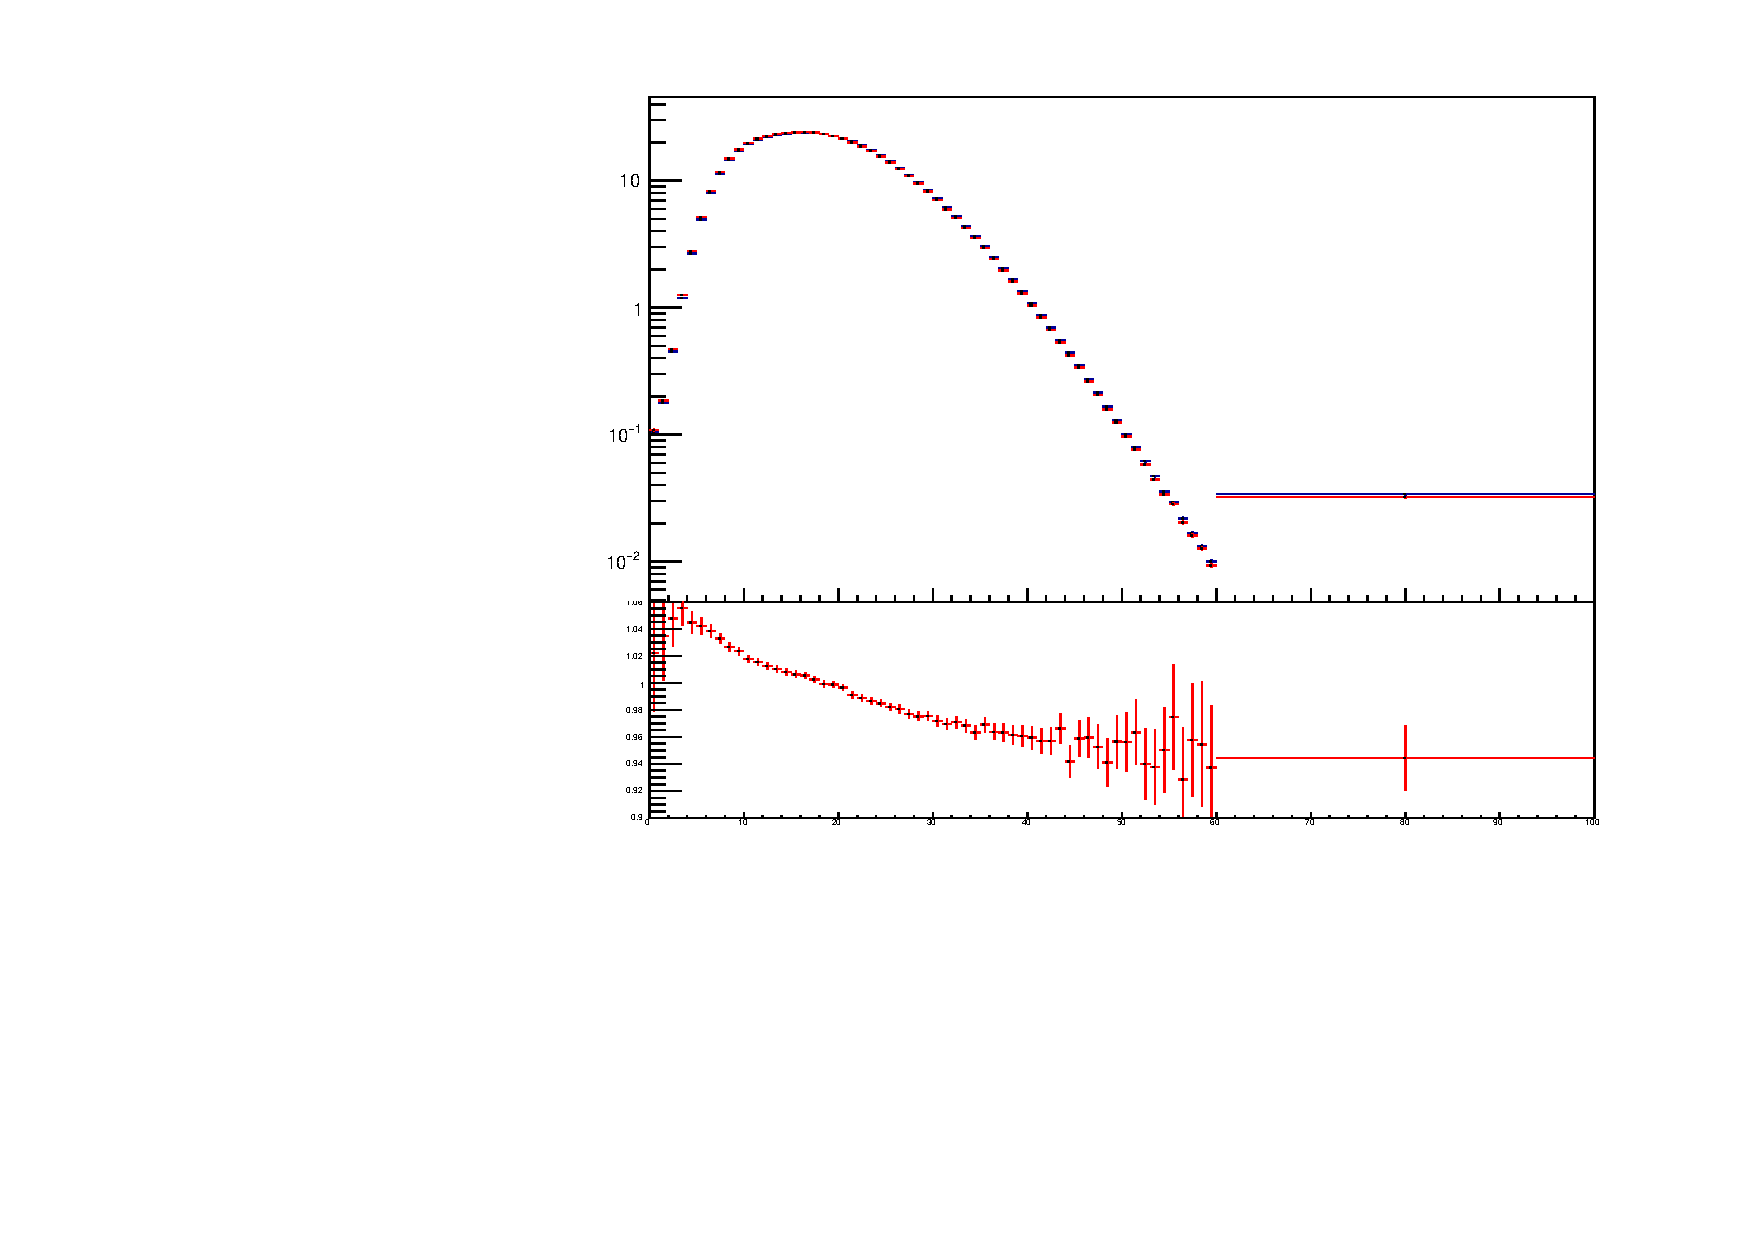
\includegraphics[width=0.48\columnwidth]{fig/Systematics/Tracking4.pdf}}     
%     \caption{Clockwise from left, the first plot shows the variation applied to account for track reconstruction efficiency. This is followed by the variation for the fake rate, the TIDE efficiency systematic and the uncertainty for weak modes in the detector alignment. As expected the variations (blue) from the nominal (red) are small, and in the case of the weak modes the effect is zero.}
%    \label{fig: ratioplots}
% \end{figure}
